\section{Anexo C: Una manera de presentar a luminus de forma diferente: Sitio web}\label{sitioweb}
Como se planteo anteriormente, inicialmente el proyecto estaba pensado para ser desarrollado como un sitio web, sin embargo, durante el desarrollo se opto por la opción de darle un comportamiento de API. esto con el fin de proporcionar una funcionalidad diferente. \\
Por lo que se puede afirmar que la API no es excluyente de el desarrollo del sitio web. y la implementación mas recomendable dependería de cada usuario final y sus necesidades. Podría trabajarse en la implementación de este sitio web para cubrir una mayor cantidad de usuarios y adaptarse de mejor manera a sus necesidades.\\
En este sentido, debido a que, ya se había pensado en este desarrollo se tiene una propuesta de como podrían diseñarse las pantallas correspondientes al sitio web por lo menos para el algoritmo KNN además de el mapa de navegación de las mismas. mismas que podrían ser usadas como referencia, o bien, ser utilizadas como tal.\\
El mapa de navegación es el siguiente:\\
\begin{figure}[H]
	\hypertarget{fig:red}{\hspace{1pt}}
	\begin{center}
		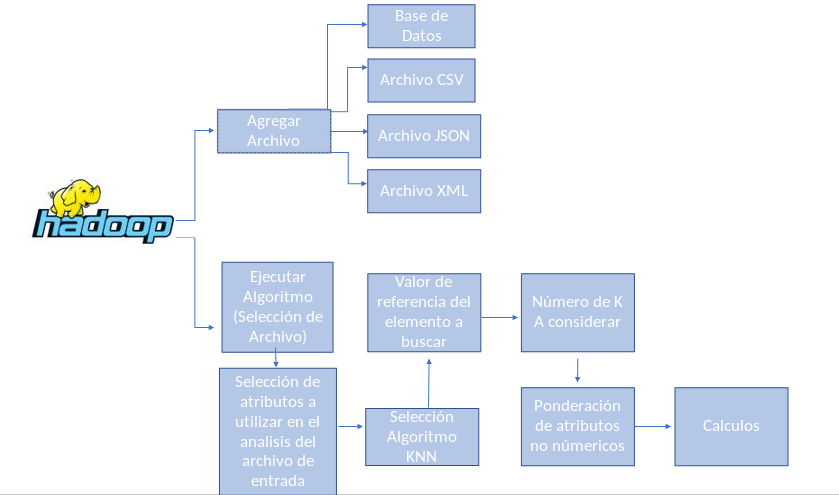
\includegraphics[width=.9\textwidth]{capitulo7/images/mapadenavegacion.png}
		\caption{Mapa de Navegación}
		\label{fig:mapanav}
	\end{center}
\end{figure}
\newpage
Se procede a explicar cada una de las pantallas que se listan en el mapa de navegación en el orden en que se mandarían a llamar, esto con el fin de que sea claro el proceso de ejecución y funcionamiento de las mismas, además de mencionar para cada una de ellas su objetivo la propuesta de visualización.\\
El diseño de pantallas propuesto, vendría directamente de las vistas que ya tiene implementadas Hadoop para su funcionamiento, es decir, se agregaría un elemento al menú de opciones de Hadoop. esto para simplificar el entendimiento de las pantallas, y como todas las tareas se realizarían de manera local no sería necesario colgarlas de ningún servicio. En este ejemplo el botón que permitiría llevar a cabo esta tarea sería \IUbutton{Funcionamiento Luminus} como se muestra en la siguiente figura:\\
\begin{figure}[H]
	\hypertarget{fig:red}{\hspace{1pt}}
	\begin{center}
		
\includegraphics[width=.9\textwidth]{capitulo7/images/menu.png}
		\caption{Funcionamiento Luminus}
		\label{fig:agre}
	\end{center}
\end{figure}
El cual, al hacer clic sobre de el, debería redirigir a las pantallas que se muestran a continuación:
\\
\textbf{\textcolor{red}{Agregar Archivo}}
\begin{figure}[H]
	\hypertarget{fig:red}{\hspace{1pt}}
	\begin{center}
		
\includegraphics[width=1\textwidth]{capitulo7/images/AgregarArchivo.png}
		\caption{Agregar Archivo}
		\label{fig:agre}
	\end{center}
\end{figure}
Esta pantalla se propone que el usuario seleccione el tipo de archivo que desea subir al HDFS. desde su directorio local, o en su defecto desde una base de datos las configuraciones de conexión a la base de datos serian hechas en pantallas posteriores.\\
Es necesario que el usuario agregue al menos un archivo de datos al HDFS antes de empezar a aplicar algoritmos ya que en caso de no existir ningún archivo sobre el HDFS, no se tendrían datos sobre los cuales trabajar.\\
Además de que es importante señalar que, los archivos que el usuario tenga en su directorio local no pueden ser leídos o manipulados por LUMINUS, ni por los algoritmos de programación, por lo que este paso es muy importante.\\
Con esto, se estaría garantizando que los archivos se encuentren sobre la red distribuida.\\
\\
\textbf{\textcolor{red}{Agregar Archivo CSV}}
\begin{figure}[H]
	\hypertarget{fig:red}{\hspace{1pt}}
	\begin{center}
		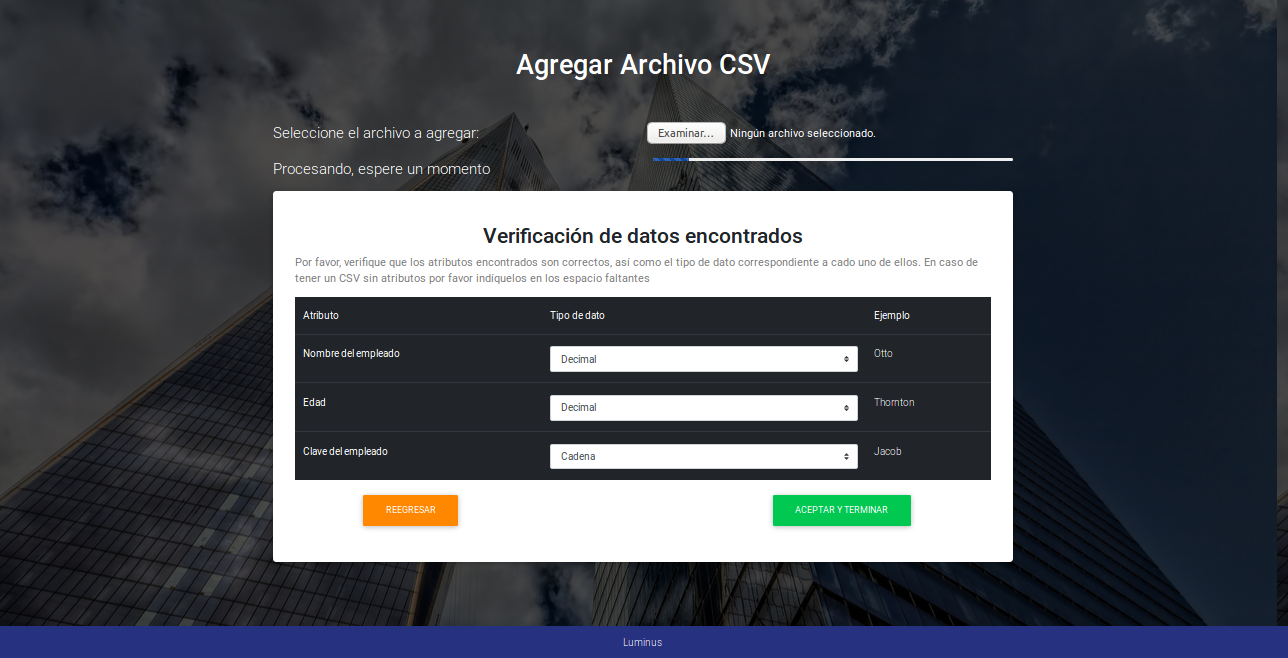
\includegraphics[width=1\textwidth]{capitulo7/images/archivoCSV.png}
		\caption{Agregar Archivo CSV}
		\label{fig:CSV}
	\end{center}
\end{figure}
En el caso que el archivo que desee subir el usuario sea de tipo CSV que son los que actualmente son soportados por la plataforma, no se tendría que realizar ningún ajuste o mejora a los algoritmos. \\
Como parte de la funcionalidad de esta pantalla se propone realizar un análisis detallado a los datos contenidos en el archivo para que, con el análisis que se haga, se le puede decir al usuario que tipo de dato se cree que contiene cada una de las columnas de su archivo, además de permitirle la opción de cambiar el tipo de dato en caso de que el tipo de dato encontrado al ser validado por el usuario este encuentre que es incorrecto. por otro lado, se propone mostrar un ejemplo de un dato contenido dentro de la columna, esto para que si el usuario no recuerda exactamente que contiene una columna, pueda darse una idea y con esto seleccionar si el tipo de dato que se encontró para esa columna efectivamente es el correcto y en caso de no serlo pueda tener los elementos para cambiarlo con toda tranquilidad.\\
Para los archivos CSV que no contienen encabezado con nombre de los atributos, se mostrara esta columna vacía y se dejará al usuario que indique su nombre.\\
Una vez terminado el proceso podrá hacer clic en uno de los dos botones listados; ya sea en \IUbutton{Aceptar y Terminar} o bien en \IUbutton{Regresar}. y esto lo determina, el hecho de que desee o no, guardar el archivo encontrado con los datos que se encuentran actualmente en la tabla mostrada en la pantalla.\\
En caso de que se presione \IUbutton{Aceptar y Terminar} esta pantalla debería validar que los tipos de dato seleccionados por el usuario puedan ser aplicados para todos los elementos que contiene cada uno de los atributos y si no lo es, mostrar uno de los elementos del atributo que no aplica para el tipo de dato introducido por el usuario, para que entonces el usuario final pueda volver a hacer la selección.\\
En caso de que todos los tipos de dato sean correctos, se debería hacer una carga de este archivo al HDFS, agregando en caso de que no lo tuviera y hayan sido introducido por el usuario los atributos correspondientes.\\
Los tipos de datos, seleccionados por el usuario, serían utilizados para alimentar los algoritmos soportados por \emph{Luminus} con los datos que cada uno de ellos soporta. y se tendría que llevar un control de estos tipos de datos, como el programador de este sitio web lo prefiera siempre y cuando no los pierda de vista para tomarlos en cuenta al momento de invocar a los programas.\\
\textbf{\textcolor{red}{Agregar XML o Agregar JSON}}
\begin{figure}[H]
	\hypertarget{fig:red}{\hspace{1pt}}
	\begin{center}
		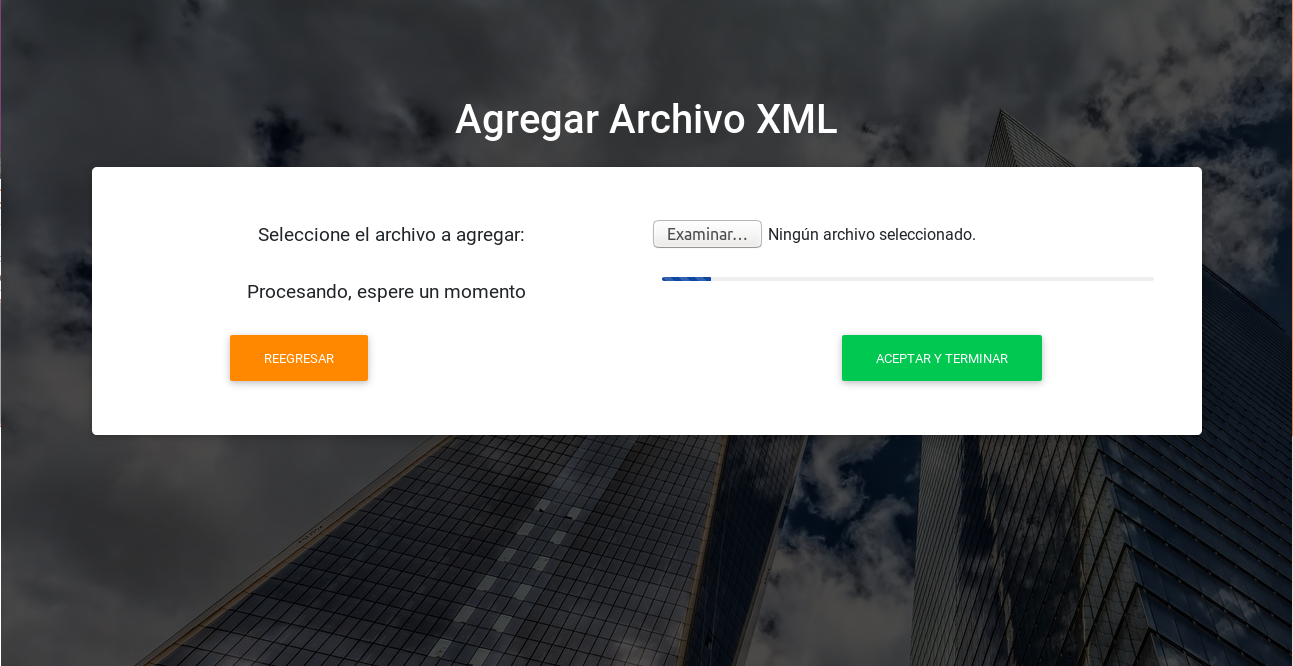
\includegraphics[width=1\textwidth]{capitulo7/images/agregarXML.png}
		\caption{Agregar Archivo XML}
		\label{fig:XML}
	\end{center}
\end{figure}
\begin{figure}[H]
	\hypertarget{fig:red}{\hspace{1pt}}
	\begin{center}
		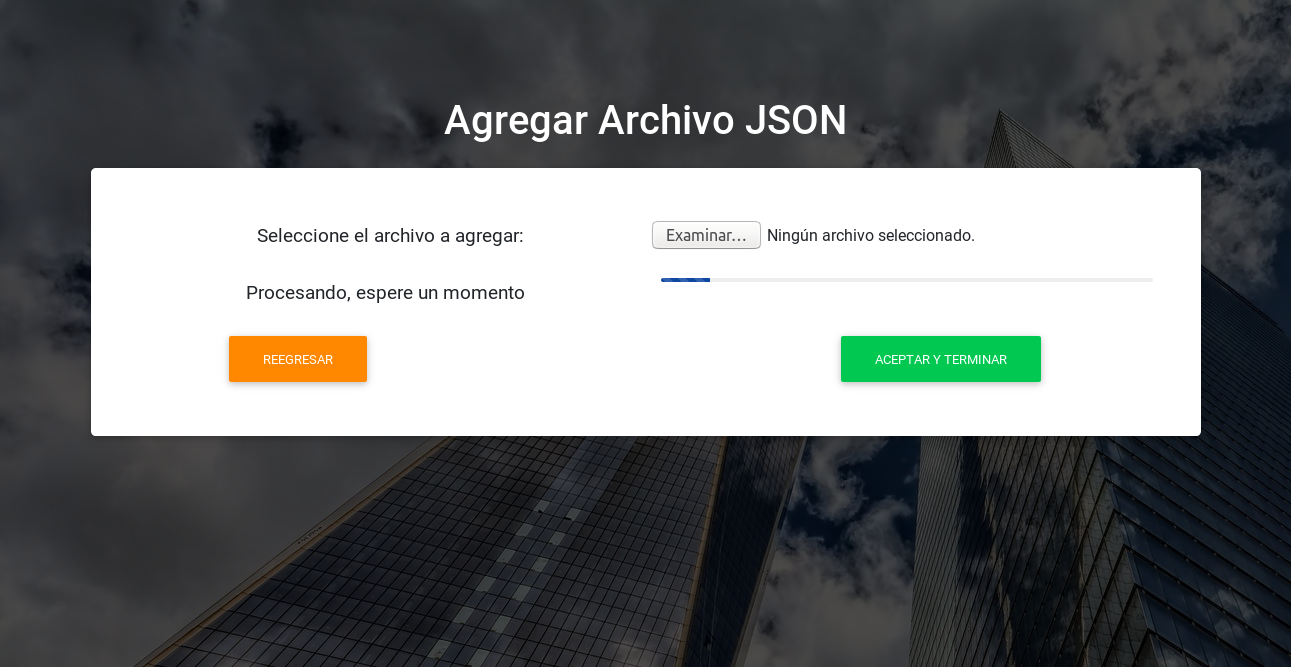
\includegraphics[width=1\textwidth]{capitulo7/images/agregarJSON.png}
		\caption{Agregar Archivo JSON}
		\label{fig:XML}
	\end{center}
\end{figure}
Estos tipos de archivo, deben ser cargado desde el directorio local del usuario del sitio web, y no debería requerir ningún tipo de configuración adicional ya que como tal, estos tipos de archivo estan diseñados de tan forma que la información que se desea conocer del archivo ya esta soportada en la propia estructura del mismo, por lo que no habría que pedir o validar detalles adicionales.\\
Sin embargo, este tipo de archivos aun no son soportados por los algoritmos implementados en \emph{Luminus} , por lo que, seria necesario realizar alguna de las siguientes opciones:
\begin{itemize}
	\item Adaptar los algoritmos que actualmente se tienen implementados en \emph{Luminus} para que sean capaces de trabajar con archivos XML y JSON
	\item Hacer un tratamiento de los datos para que a pesar de que su origen sea un tipo de archivo distinto (XML, JSON) puedan ser tratados como un CSV y soportados por los algoritmos. 
\end{itemize} 
Sin embargo, sin importar la solución que se escoja será necesario realizar la subida de los archivos al directorio del HDFS.\\

\textbf{\textcolor{red}{Agregar Base de Datos}}
\begin{figure}[H]
	\hypertarget{fig:red}{\hspace{1pt}}
	\begin{center}
		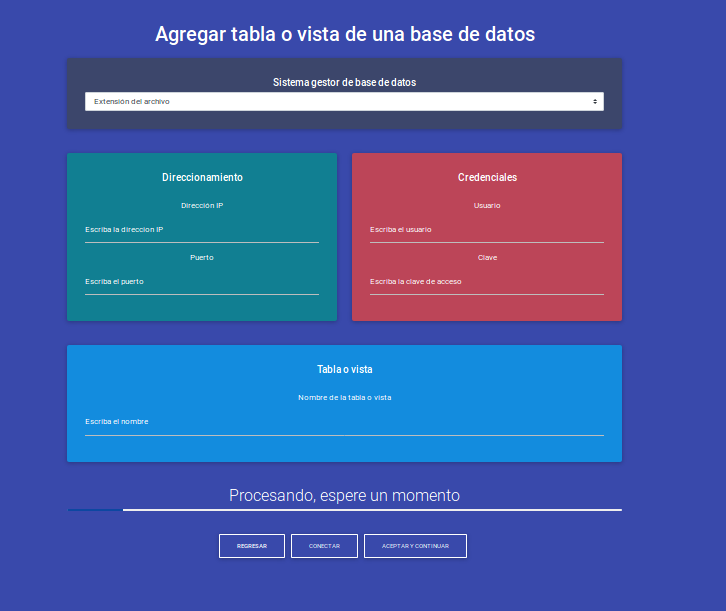
\includegraphics[width=1.1\textwidth]{capitulo7/images/basededatos.png}
		\caption{Agregar Tabla o Vista de una Base de Datos}
		\label{fig:Tabla}
	\end{center}
\end{figure}
Algunas veces los usuarios, tendrán sus datos en bases de datos relacionales convencionales. ya que es una manera muy común que utilizan las empresas para el tratamiento de sus datos, en este caso, se puede destinar una tabla o una vista para poder trabajar con los datos que estas nos arrojan.\\
La vista, en su caso, le permitiría al usuario final, incluir solo algunos campos de una determinada tabla, o bien datos de varias tablas haciendo las uniones entre las tablas que este necesite. \\
Por lo que una vez que el usuario tuviera lista su vista o bien su tabla, podrá en esta pantalla ingresar las credenciales de su base de datos, las cuales son:
\begin{itemize}
	\item Dirección IP
	\item Puerto donde corre la base de datos
	\item Nombre de usuario
	\item Clave de este usuario dentro de la base de datos 
\end{itemize} 
Bases de datos de diferentes manejadores, pueden establecer una conexión unicamente con estos 4 datos por lo que se considera que estos podrían ser suficientes para testear una conexión.\\ 
Antes de realizar el Testeo, será necesario que el usuario indique cual es el nombre de la tabla o vista con la que desea conectarse, después de esto. se puede verificar que la conexión a la base de datos es valida y continuar con el copiado de la tabla o de la vista dentro de el HDFS.\\
La implementación para base de datos, no es soportada actualmente por los algoritmos de clasificación programados, por lo que se tendría que implementar alguna de las siguientes soluciones:\\
\begin{itemize}
	\item Adaptar los algoritmos de \emph{Luminus} para que sean capaces de trabajar con archivos originarios de una base de datos ya sea una tabla o una vista.
	\item Hacer un tratamiento de los datos para que a pesar de que su origen sea un tipo de archivo distinto (Base de datos) puedan ser tratados como un CSV y soportados por los algoritmos. 
\end{itemize}  
En este caso, es necesario considerar, cuantos tipos de bases de datos diferentes pueden ser soportados por los algoritmos debido a que cada base de datos que se maneje tiene diferentes formas de exportar sus datos, y este comportamiento deberá ser considerado al momento de manejarlos.\\
\textbf{\textcolor{red}{Ejecutar algoritmo (Selección de Archivo)}}
\begin{figure}[H]
	\hypertarget{fig:red}{\hspace{1pt}}
	\begin{center}
		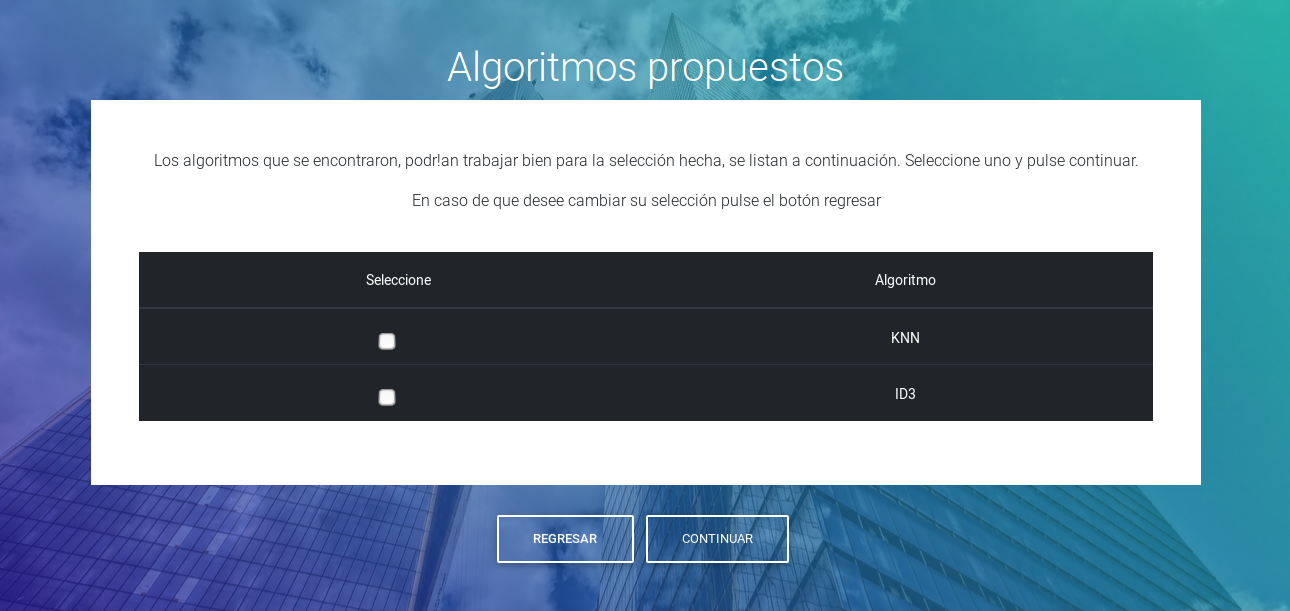
\includegraphics[width=1\textwidth]{capitulo7/images/algoritmospro.png}
		\caption{Algoritmos Propuestos}
		\label{fig:algo}
	\end{center}
\end{figure}
En esta pantalla se pretende presentar todos los tipos de algoritmos que pueden ser soportados por la aplicación, por el momento ID3 y KNN, en caso de que, se desarrollen mas algoritmos podrían ser listados desde esta misma pantalla.\\
Sería necesario que el usuario seleccionará del listado mostrado el algoritmo que desea ejecutar.\\
\textbf{\textcolor{red}{Algoritmo KNN}}
\\
A continuación se muestra un ejemplo de como podría operar el algoritmo KNN en esta implementación. no se tiene una propuesta para el algoritmo ID3 pero la lógica que estos debería ser la misma.\\
Si se alcanza a visualizar la forma en que se pretende presentar este algoritmo, podría diseñarse una solución para cada uno de los algoritmos que sean implementados.\\
\textbf{\textcolor{red}{Ejecutar Algoritmo}}
\\
\begin{figure}[H]
	\hypertarget{fig:red}{\hspace{1pt}}
	\begin{center}
		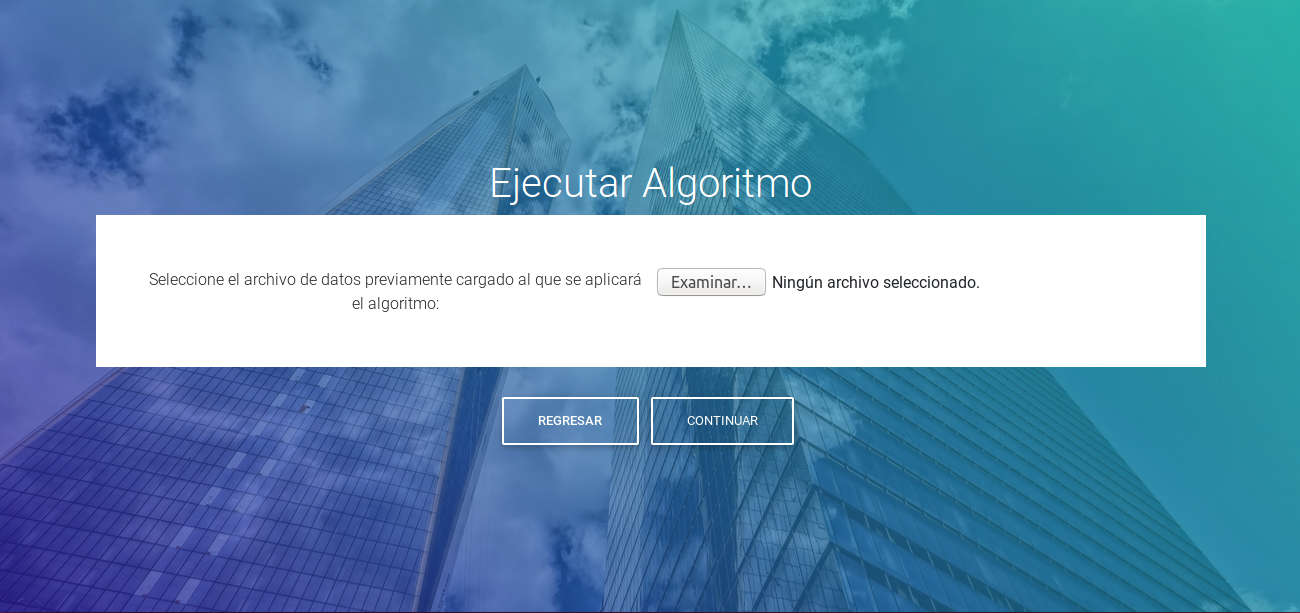
\includegraphics[width=1\textwidth]{capitulo7/images/seleccione.png}
		\caption{Ejecutar Algoritmo}
		\label{fig:seleccione}
	\end{center}
\end{figure}
En este caso, se buscará en el HDFS, el archivo que contiene los datos que se desean aplicar al algoritmo KNN, ya que, el HDFS puede contener mas de un archivo de datos. pero será necesario distinguir cual de ellos sera utilizado para cada ejecución. 
Una vez que este se seleccione se presionaría \IUbutton{Continuar}.\\
\\
\newpage
\textbf{\textcolor{red}{Selección de atributos a utilizar en el ánalisis del archivo de entrada}}
\begin{figure}[H]
	\hypertarget{fig:red}{\hspace{1pt}}
	\begin{center}
		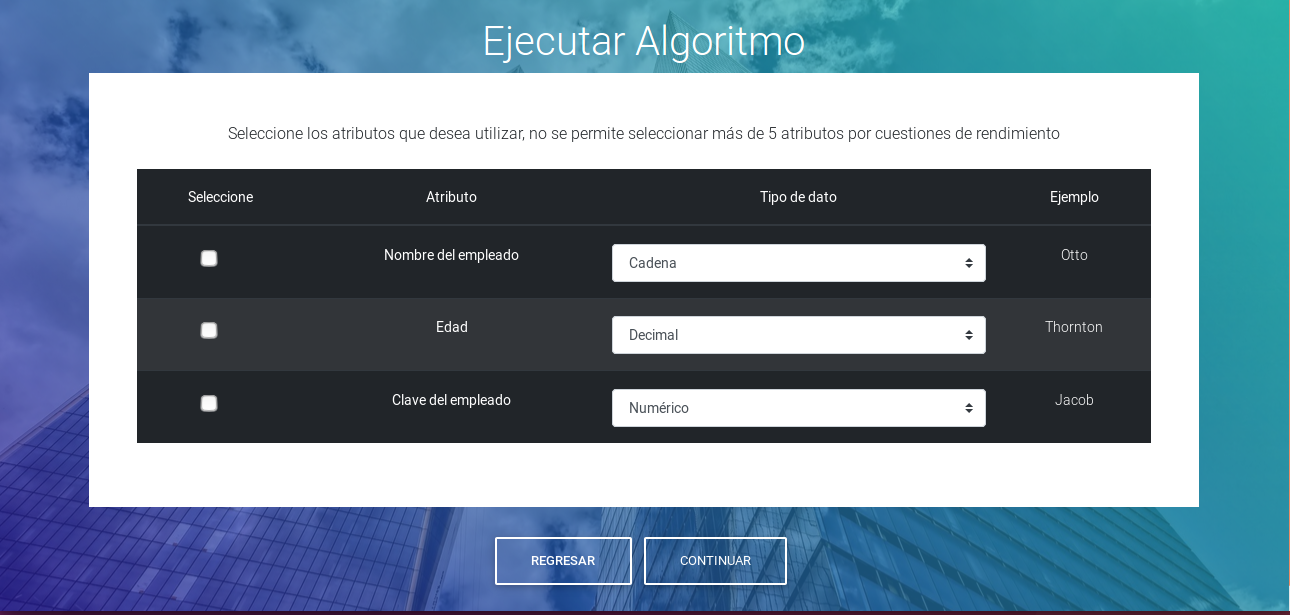
\includegraphics[width=1\textwidth]{capitulo7/images/ejecutar2.png}
		\caption{Selección de atributos}
		\label{fig:seleccioneatr}
	\end{center}
\end{figure}
En esta pantalla, se muestran los atributos contenidos dentro del archivo de configuraciones, para que el usuario seleccione los que desea utilizar como parte del procesamiento. \\
Se propone restringir a que no sea posible seleccionar mas de 5 atributos, ya que entre mas atributos se incluyan en el algoritmo mas complejo se vuelve su procesamiento, sin embargo, podría no ser restringido y seguiría operando de manera correcta.\\
Nuevamente, si el usuario desea cambiar el tipo de dato, debería ser permitido. ya que quizá desee tratar el mismo dato de diferentes maneras para diferentes algoritmos. Pero sería recomendable mantener los que selecciono anteriormente, para que solo requiera hacer los cambios para los atributos que tengan modificaciones y el resto de ellos no tenga que volver a introducirlos cada que quiera ejecutar un algoritmo.\\
\newpage
\textbf{\textcolor{red}{Valor de referencia del elemento a buscar}}
\begin{figure}[H]
	\hypertarget{fig:red}{\hspace{1pt}}
	\begin{center}
		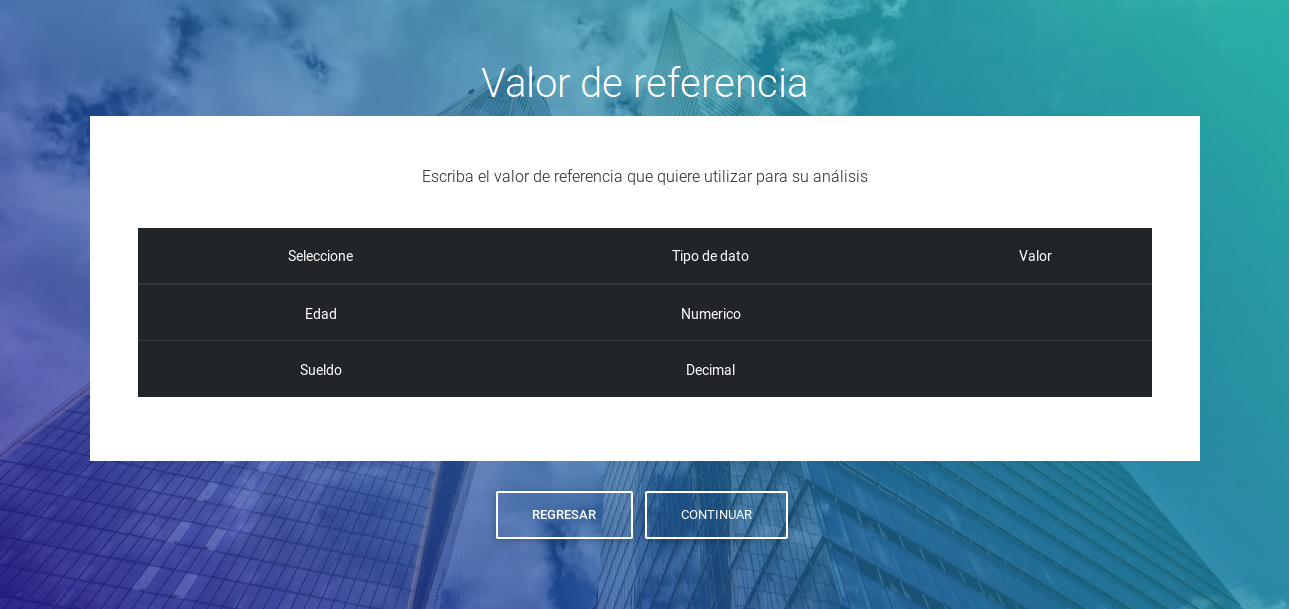
\includegraphics[width=1\textwidth]{capitulo7/images/referencia.png}
		\caption{Valor de Referencia}
		\label{fig:ref}
	\end{center}
\end{figure}
Para todos los datos seleccionados en la pantalla anterior se tiene que dar un valor de referencia para el análisis, este servirá para encontrar el número de vecinos mas cercanos. el valor que se ingrese debe ser del mismo tipo de dato, seleccionado en la pantalla anterior.\\ 
\textbf{\textcolor{red}{Número de K a considerar}}
\begin{figure}[H]
	\hypertarget{fig:red}{\hspace{1pt}}
	\begin{center}
		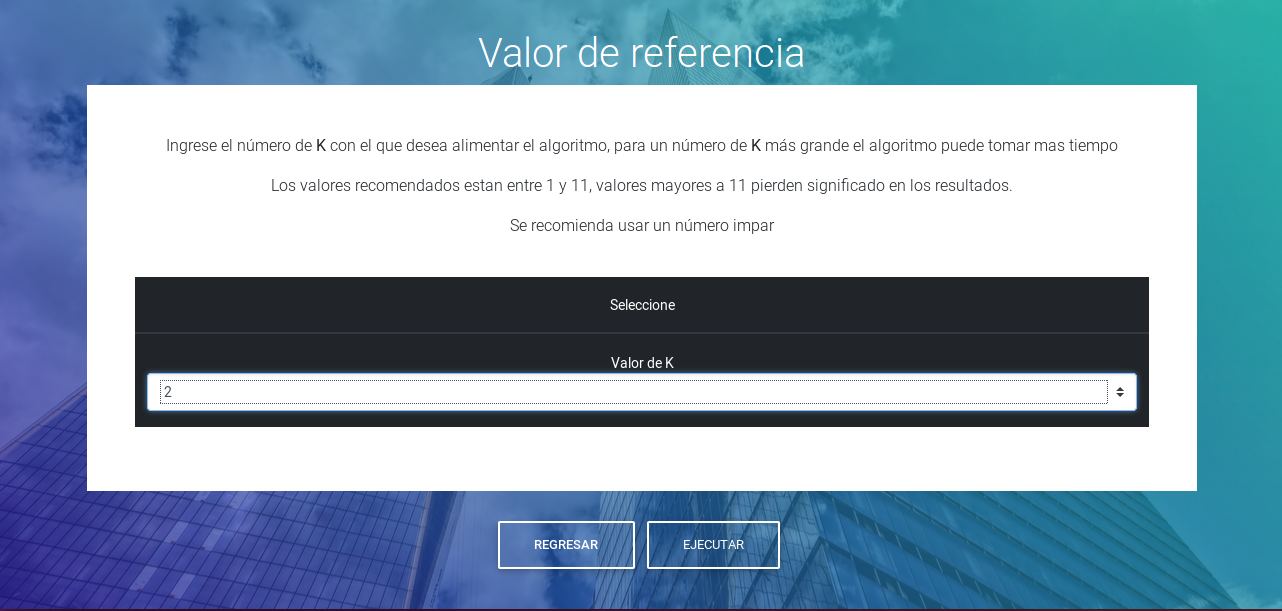
\includegraphics[width=1\textwidth]{capitulo7/images/valorK.png}
		\caption{Valor K}
		\label{fig:ref}
	\end{center}
\end{figure}  
En este caso, para obtener los valores se selecciona un numero de K valido, se recomienda seleccionar este valor entre 0 y 11. para hacer mas simple el análisis. ya que valores de k superiores a 11 la información empieza a perder valor.\\
esta pantalla unicamente permite seleccionar el valor mas apropiado para esta variable.\\
\textbf{\textcolor{red}{Ponderación de atributos no númericos}}
\\
\begin{figure}[H]
	\hypertarget{fig:red}{\hspace{1pt}}
	\begin{center}
		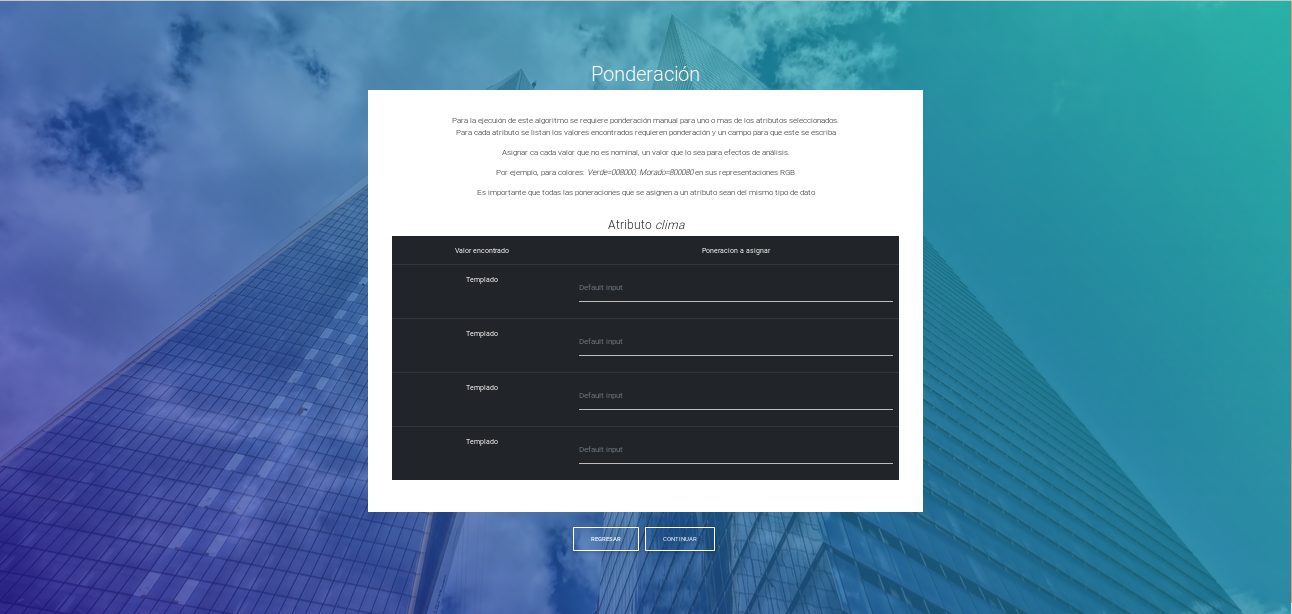
\includegraphics[width=1\textwidth]{capitulo7/images/ponderacion.png}
		\caption{Ponderación}
		\label{fig:pond}
	\end{center}
\end{figure}  
Un elemento que se puede agregar a las consideraciones hechas es la ponderación de atributos no numéricos.\\
Se trata de valores, que no pueden ser trabajados de manera inmediata por los algoritmos, por lo que hay que asignarles un valor de manera manual a cada uno de los elementos del atributo. Esto es viable mientras que, el número de elementos dentro de un atributo no haya crecido demasiado, ya que para atributos con muchas opciones esto se volvería muy pesado.\\
Sería necesario establecer un número máximo de valores diferentes permitidos para que, atributos que tengan mas elementos que ese numero establecido no puedan ser configurados de esa forma.\\
Todas las ponderaciones que se establezcan, deben de ser del mismo tipo de dato, y debe de configurarse el archivo de tal forma que cuando se pase a los algoritmos pueda leer los datos ponderados para que el algoritmo que se pretende utilizar funcione de manera correcta.\\
Al inicio de la sección Trabajo a Futuro se detalla un poco mas acerca de que significa hacer las ponderaciones y se detalla un ejemplo en caso de que se requiera mas información al respecto.\\
\newpage
\textbf{\textcolor{red}{Ejecución del algoritmo}}
\\
\begin{figure}[H]
	\hypertarget{fig:red}{\hspace{1pt}}
	\begin{center}
		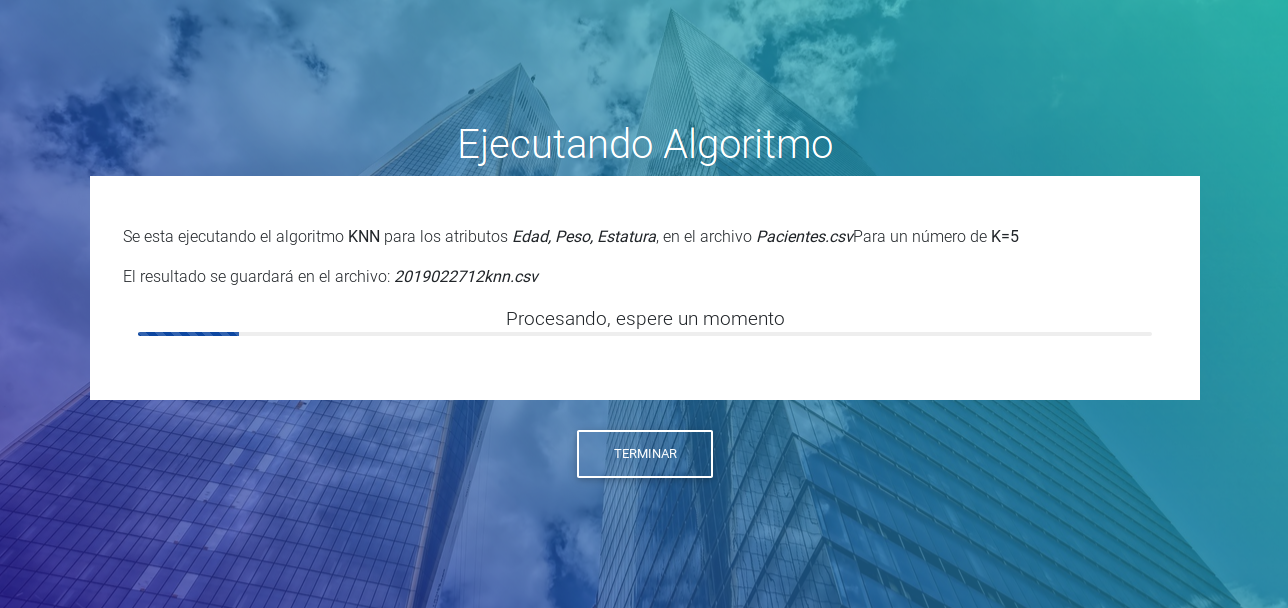
\includegraphics[width=1\textwidth]{capitulo7/images/ejecutar.png}
		\caption{Ejecución del algoritmo}
		\label{fig:pond}
	\end{center}
\end{figure}
Cuando se realicen todas las configuraciones necesarias, entonces se procede a ejecutar el algoritmo pasandole las configuraciones establecidas y se devuelve al usuario un archivo de salidas en el formato mas recomendable para el algoritmo que se este ejecutando. con los resultados obtenidos de la ejecución del algoritmo.